\documentclass[10pt,a4paper]{article}

% --- Packages ---
\usepackage[utf8]{inputenc}
\usepackage[T1]{fontenc}
\usepackage[margin=0.65in, top=0.85in, bottom=0.75in, headheight=20pt]{geometry}
\usepackage[table]{xcolor}
\usepackage{helvet}
\renewcommand{\familydefault}{\sfdefault}
\usepackage{microtype}
\usepackage{amsmath,amssymb}
\usepackage{booktabs}
\usepackage{tabularx}
\usepackage{colortbl}
\usepackage{tcolorbox}
\tcbuselibrary{skins,breakable}
\usepackage{tikz}
\usetikzlibrary{positioning,calc,shapes.geometric,backgrounds,patterns}
\usepackage{fontawesome5}
\usepackage{enumitem}
\usepackage{fancyhdr}
\usepackage{lastpage}
\usepackage{titlesec}
\usepackage[colorlinks=true,linkcolor=BlueAccent,urlcolor=BlueAccent,pdfstartview=FitH]{hyperref}

% --- Color Palette Definitions (No trailing spaces) ---
\definecolor{NavyPrimary}{HTML}{0F172A}
\definecolor{BlueAccent}{HTML}{0284C7}
\definecolor{TealSuccess}{HTML}{0D9488}
\definecolor{DarkText}{HTML}{1E293B}
\definecolor{LightBg}{HTML}{F8FAFC}
\definecolor{CardBg}{HTML}{F1F5F9}
\definecolor{BorderColor}{HTML}{E2E8F0}
\definecolor{MutedText}{HTML}{64748B}
\definecolor{AlertRed}{HTML}{DC2626}
\definecolor{GoldHighlight}{HTML}{D97706}

% --- Page Setup & Header/Footer ---
\pagestyle{fancy}
\fancyhf{}
\renewcommand{\headrulewidth}{0.4pt}
\renewcommand{\headrule}{{\color{BorderColor}\hrule width\headwidth height 0.4pt}}
\renewcommand{\footrulewidth}{0.4pt}
\renewcommand{\footrule}{{\color{BorderColor}\hrule width\headwidth height 0.4pt}}

\fancyhead[L]{\small\bfseries\color{NavyPrimary} NEXA SYSTEMS INC. \ \smallextra{\color{MutedText}| \ Enterprise SaaS Financial Summary}}
\fancyhead[R]{\small\color{MutedText} CONFIDENTIAL \ \smallextra{\color{BorderColor}|} \ FY2026--FY2028 PLAN}
\fancyfoot[L]{\small\color{MutedText} Prepared by: Corporate FP\&A Group \ -- \ Nexa Systems}
\fancyfoot[R]{\small\color{NavyPrimary}\bfseries Page \thepage\ of \pageref{LastPage}}

\newcommand{\smallextra}[1]{{\small #1}}

% --- Section Styling ---
\titleformat{\section}
  {\color{NavyPrimary}\normalfont\large\bfseries}
  {}
  {0pt}
  {\tikz[baseline=(char.base)]\node[fill=BlueAccent,inner sep=2pt,text=white,font=\small\bfseries,rounded corners=1pt] (char) {\thesection}; \ }

\titleformat{\subsection}
  {\color{NavyPrimary}\normalfont\normalsize\bfseries}
  {}
  {0pt}
  {}

\titlespacing*{\section}{0pt}{14pt}{8pt}
\titlespacing*{\subsection}{0pt}{10pt}{4pt}

% --- Custom tcolorbox Styles ---
\tcbset{
  kpicard/.style={
    enhanced,
    colback=LightBg,
    colframe=BorderColor,
    arc=4pt,
    boxrule=0.8pt,
    top=8pt, bottom=8pt, left=8pt, right=8pt,
    boxsep=0pt
  },
  calloutbox/.style={
    enhanced,
    colback=CardBg,
    colframe=NavyPrimary,
    arc=3pt,
    boxrule=0.5pt,
    leftrule=3.5pt,
    top=8pt, bottom=8pt, left=10pt, right=10pt
  },
  tablebox/.style={
    enhanced,
    colback=white,
    colframe=BorderColor,
    arc=3pt,
    boxrule=0.6pt,
    top=4pt, bottom=4pt, left=4pt, right=4pt
  }
}

% --- Helper Macros ---
\newcommand{\kpival}[3]{%
  {\raggedright
  {\tiny\bfseries\color{MutedText}\uppercase{#1}}\par\vspace{2pt}
  {\Large\bfseries\color{NavyPrimary}#2}\par\vspace{2pt}
  {\small\bfseries#3}\par}%
}

\newcommand{\positivechange}[1]{\color{TealSuccess}\faArrowUp\ #1}
\newcommand{\negativechange}[1]{\color{AlertRed}\faArrowDown\ #1}
\newcommand{\neutralchange}[1]{\color{MutedText}#1}
\newcommand{\xs}{\tiny}

\begin{document}

% ==========================================
% PAGE 1: EXECUTIVE SUMMARY & CORE METRICS
% ==========================================

% --- Header Title Block ---
\begin{tcolorbox}[enhanced, colback=NavyPrimary, colframe=NavyPrimary, arc=4pt, top=12pt, bottom=12pt, left=14pt, right=14pt]
  \begin{minipage}[c]{0.66\textwidth}
    \color{white}
    {\huge\bfseries Enterprise SaaS Financial Summary}\par\vspace{4pt}
    {\large\color{BlueAccent}\bfseries Nexa Systems Inc. \ -- \ FY2026 Strategic Plan \& Multi-Year Forecast}
  \end{minipage}%
  \hfill
  \begin{minipage}[c]{0.30\textwidth}
    \color{white}\raggedleft
    {\small\bfseries Board \& Executive Report}\par
    {\footnotesize\color{BorderColor} Date: July 2026}\par
    {\footnotesize\color{BorderColor} Model Version: 4.2 (Base Case)}
  \end{minipage}
\end{tcolorbox}

\vspace{6pt}

% --- Executive KPI Dashboard (2x3 Minipage Grid) ---
\noindent
\begin{minipage}[t]{0.31\textwidth}
  \begin{tcolorbox}[kpicard]
    \kpival{Annual Recurring Revenue (ARR)}{\$42.8M}{\positivechange{+38.5\% YoY (Target: \$40.0M)}}
  \end{tcolorbox}
\end{minipage}%
\hfill
\begin{minipage}[t]{0.31\textwidth}
  \begin{tcolorbox}[kpicard]
    \kpival{Net Revenue Retention (NRR)}{118.4\%}{\positivechange{+240 bps vs FY25 (Ent: 124\%)}}
  \end{tcolorbox}
\end{minipage}%
\hfill
\begin{minipage}[t]{0.31\textwidth}
  \begin{tcolorbox}[kpicard]
    \kpival{CAC Payback Period}{11.2 mos}{\positivechange{Improved from 13.8 mos YoY}}
  \end{tcolorbox}
\end{minipage}

\par\vspace{6pt}

\noindent
\begin{minipage}[t]{0.31\textwidth}
  \begin{tcolorbox}[kpicard]
    \kpival{LTV / CAC Ratio}{4.8x}{\positivechange{Target: >3.5x (Benchmark 4.0x)}}
  \end{tcolorbox}
\end{minipage}%
\hfill
\begin{minipage}[t]{0.31\textwidth}
  \begin{tcolorbox}[kpicard]
    \kpival{Gross Margin (Subscription)}{78.2\%}{\positivechange{+180 bps Cloud Infra Eff.}}
  \end{tcolorbox}
\end{minipage}%
\hfill
\begin{minipage}[t]{0.31\textwidth}
  \begin{tcolorbox}[kpicard]
    \kpival{Rule of 40 Score}{52.7\%}{\positivechange{Rev Growth 38.5\% + FCF 14.2\%}}
  \end{tcolorbox}
\end{minipage}

\vspace{10pt}

% --- Executive Commentary Callout ---
\begin{tcolorbox}[calloutbox]
  \noindent\textbf{\color{NavyPrimary}\faFile\ Executive Summary \& Strategic Growth Drivers}
  \par\vspace{4pt}
  \small\color{DarkText}
  Nexa Systems demonstrates exceptional operational leverage and accelerating growth entering FY2026. Key growth across our flagship platforms -- \textbf{Vertex AI Governance} and \textbf{Synapse Data Engine} -- drove a 38.5\% ARR expansion to \$42.8M. Enterprise deal velocity increased significantly, pushing Average Contract Value (ACV) from \$68k to \$94k. Net Revenue Retention reached 118.4\%, underpinned by enterprise expansion seats and cross-selling the newly launched Meridian Analytics module. Free Cash Flow margin expanded to 14.2\%, confirming path-to-profitability targets while sustaining top-quartile Rule of 40 performance (52.7\%).
\end{tcolorbox}

\vspace{8pt}

% --- Summary Financial Statement (Table) ---
\section{Consolidated Summary Financial Statement (FY2024 -- FY2028E)}

\noindent
\begin{tcolorbox}[tablebox]
  \small
  \rowcolors{2}{LightBg}{white}
  \begin{tabularx}{\textwidth}{X r r r r r r}
    \toprule
    \textbf{\color{NavyPrimary}Financial Metric (\$ in Millions)} & \textbf{FY2024} & \textbf{FY2025} & \textbf{FY2026E} & \textbf{FY2027E} & \textbf{FY2028E} & \textbf{CAGR (24-28)} \\
    \midrule
    Subscription Revenue & \$22.4 & \$30.2 & \$41.5 & \$57.8 & \$79.6 & 37.3\% \\
    Professional Services & \$1.8 & \$2.1 & \$2.7 & \$3.4 & \$4.2 & 23.6\% \\
    \textbf{Total Revenue} & \textbf{\$24.2} & \textbf{\$32.3} & \textbf{\$44.2} & \textbf{\$61.2} & \textbf{\$83.8} & \textbf{36.4\%} \\
    \quad \textit{\% YoY Revenue Growth} & \textit{41.2\%} & \textit{33.5\%} & \textit{36.8\%} & \textit{38.5\%} & \textit{36.9\%} & \textit{--} \\
    \midrule
    Cost of Goods Sold (COGS) & \$5.8 & \$7.2 & \$9.2 & \$12.1 & \$15.8 & 28.4\% \\
    \textbf{Gross Profit} & \textbf{\$18.4} & \textbf{\$25.1} & \textbf{\$35.0} & \textbf{\$49.1} & \textbf{\$68.0} & \textbf{38.7\%} \\
    \quad \textit{\% Gross Margin} & \textit{76.0\%} & \textit{77.7\%} & \textit{79.2\%} & \textit{80.2\%} & \textit{81.1\%} & \textit{+510 bps} \\
    \midrule
    Research \& Development (R\&D) & \$7.1 & \$9.2 & \$11.8 & \$15.2 & \$19.8 & 29.2\% \\
    Sales \& Marketing (S\&M) & \$9.8 & \$12.4 & \$15.5 & \$20.2 & \$26.1 & 27.7\% \\
    General \& Administrative (G\&A) & \$3.2 & \$3.9 & \$4.8 & \$6.0 & \$7.6 & 24.1\% \\
    \textbf{Total Operating Expenses} & \textbf{\$20.1} & \textbf{\$25.5} & \textbf{\$32.1} & \textbf{\$41.4} & \textbf{\$53.5} & \textbf{27.7\%} \\
    \midrule
    \textbf{EBITDA} & \textbf{-\$1.7} & \textbf{-\$0.4} & \textbf{\$2.9} & \textbf{\$7.7} & \textbf{\$14.5} & \textbf{N/A} \\
    \quad \textit{\% EBITDA Margin} & \textit{-7.0\%} & \textit{-1.2\%} & \textit{6.6\%} & \textit{12.6\%} & \textit{17.3\%} & \textit{+2430 bps} \\
    Free Cash Flow (FCF) & -\$2.4 & -\$0.8 & \$6.3 & \$11.2 & \$18.4 & N/A \\
    \textbf{\% FCF Margin} & \textbf{-9.9\%} & \textbf{-2.5\%} & \textbf{14.2\%} & \textbf{18.3\%} & \textbf{22.0\%} & \textbf{+3190 bps} \\
    \bottomrule
  \end{tabularx}
\end{tcolorbox}

\vfill
\pagebreak

% ==========================================
% PAGE 2: UNIT ECONOMICS & ARR WATERFALL
% ==========================================

\section{ARR Waterfall \& Customer Dynamics}

\noindent
\begin{minipage}[t]{0.48\textwidth}
  \subsection{ARR Bridge \& Growth Waterfall}
  \vspace{-2pt}
  \begin{tcolorbox}[tablebox]
    \small
    \rowcolors{2}{LightBg}{white}
    \begin{tabularx}{\textwidth}{X r r}
      \toprule
      \textbf{ARR Component} & \textbf{FY2025} & \textbf{FY2026E} \\
      \midrule
      \textbf{Beginning ARR} & \textbf{\$30.9M} & \textbf{\$42.8M} \\
      \quad (+) New Logo ARR & +\$9.2M & +\$12.5M \\
      \quad (+) Customer Expansion ARR & +\$5.1M & +\$7.4M \\
      \quad (-) Contraction ARR & -\$1.1M & -\$1.3M \\
      \quad (-) Logo Churn ARR & -\$1.3M & -\$1.6M \\
      \midrule
      \textbf{Ending ARR} & \textbf{\$42.8M} & \textbf{\$59.8M} \\
      \quad \textit{Net New ARR} & \textit{+\$11.9M} & \textit{+\$17.0M} \\
      \quad \textit{Gross Dollar Retention (GDR)} & \textit{92.2\%} & \textit{93.2\%} \\
      \quad \textit{Net Dollar Retention (NDR)} & \textit{118.4\%} & \textit{121.0\%} \\
      \bottomrule
    \end{tabularx}
  \end{tcolorbox}
\end{minipage}%
\hfill
\begin{minipage}[t]{0.49\textwidth}
  \subsection{Unit Economics by Target Segment}
  \vspace{-2pt}
  \begin{tcolorbox}[tablebox]
    \small
    \rowcolors{2}{LightBg}{white}
    \begin{tabularx}{\textwidth}{X r r}
      \toprule
      \textbf{Metric} & \textbf{Mid-Market} & \textbf{Enterprise} \\
      \midrule
      Customer Count & 342 & 118 \\
      Average Contract Value (ACV) & \$38,500 & \$145,000 \\
      Average Sales Cycle & 42 Days & 115 Days \\
      Fully Loaded CAC & \$24,200 & \$112,000 \\
      Gross Margin & 76.5\% & 81.2\% \\
      Average Customer Lifespan & 5.2 Yrs & 7.8 Yrs \\
      Customer LTV & \$153,000 & \$918,000 \\
      \midrule
      \textbf{LTV / CAC Ratio} & \textbf{6.3x} & \textbf{8.2x} \\
      \textbf{CAC Payback (Months)} & \textbf{9.8 mos} & \textbf{11.4 mos} \\
      \bottomrule
    \end{tabularx}
  \end{tcolorbox}
\end{minipage}

\vspace{12pt}

% --- TikZ Visual Diagram: ARR Growth Trajectory ---
\subsection{Multi-Year ARR Growth \& Efficiency Trajectory}

\begin{center}
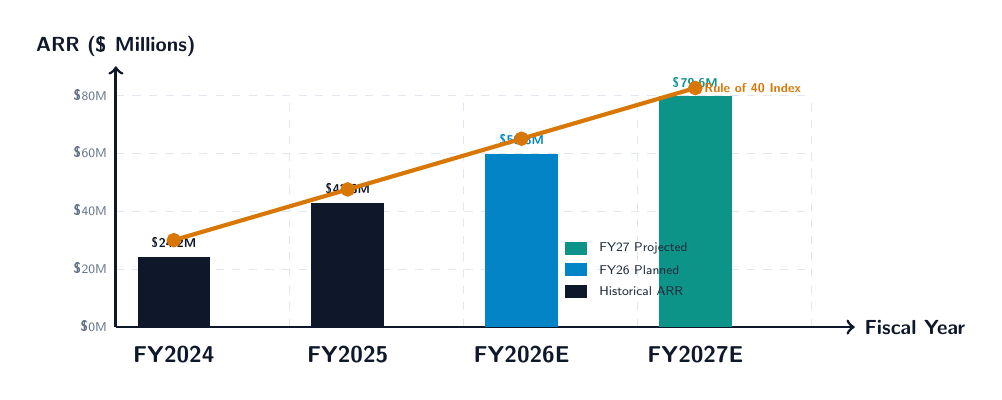
\begin{tikzpicture}[scale=0.92, transform shape]
  % Grid lines
  \draw[color=BorderColor, dashed, line width=0.4pt] (0,0) grid [ystep=0.8, xstep=2.4] (9.6,3.2);
  
  % Axes
  \draw[->, color=NavyPrimary, line width=1pt] (0,0) -- (10.2,0) node[right, font=\footnotesize\bfseries] {Fiscal Year};
  \draw[->, color=NavyPrimary, line width=1pt] (0,0) -- (0,3.6) node[above, font=\footnotesize\bfseries] {ARR (\$ Millions)};
  
  % Y-Axis Labels
  \node[left, font=\tiny\color{MutedText}] at (0,0.0) {\$0M};
  \node[left, font=\tiny\color{MutedText}] at (0,0.8) {\$20M};
  \node[left, font=\tiny\color{MutedText}] at (0,1.6) {\$40M};
  \node[left, font=\tiny\color{MutedText}] at (0,2.4) {\$60M};
  \node[left, font=\tiny\color{MutedText}] at (0,3.2) {\$80M};
  
  % X-Axis Labels
  \node[below, font=\small\bfseries\color{NavyPrimary}] at (0.8,-0.15) {FY2024};
  \node[below, font=\small\bfseries\color{NavyPrimary}] at (3.2,-0.15) {FY2025};
  \node[below, font=\small\bfseries\color{NavyPrimary}] at (5.6,-0.15) {FY2026E};
  \node[below, font=\small\bfseries\color{NavyPrimary}] at (8.0,-0.15) {FY2027E};
  
  % Bars (ARR Breakdown: Base + Expansion)
  % FY24: 24.2M -> y=0.968
  \draw[fill=NavyPrimary, draw=none] (0.3,0) rectangle (1.3,0.968);
  \node[above, font=\xs\bfseries\color{NavyPrimary}] at (0.8,0.968) {\$24.2M};
  
  % FY25: 42.8M -> y=1.712
  \draw[fill=NavyPrimary, draw=none] (2.7,0) rectangle (3.7,1.712);
  \node[above, font=\xs\bfseries\color{NavyPrimary}] at (3.2,1.712) {\$42.8M};
  
  % FY26E: 59.8M -> y=2.392
  \draw[fill=BlueAccent, draw=none] (5.1,0) rectangle (6.1,2.392);
  \node[above, font=\xs\bfseries\color{BlueAccent}] at (5.6,2.392) {\$59.8M};
  
  % FY27E: 79.6M -> y=3.184
  \draw[fill=TealSuccess, draw=none] (7.5,0) rectangle (8.5,3.184);
  \node[above, font=\xs\bfseries\color{TealSuccess}] at (8.0,3.184) {\$79.6M};
  
  % Trend line overlay (Magic Number)
  \draw[color=GoldHighlight, line width=1.5pt, mark=*] plot coordinates {(0.8, 1.2) (3.2, 1.9) (5.6, 2.6) (8.0, 3.3)};
  \node[color=GoldHighlight, right, font=\tiny\bfseries] at (8.0,3.3) {Rule of 40 Index};
  
  % Legend
  \begin{scope}[shift={(6.2,0.4)}]
    \draw[fill=NavyPrimary, draw=none] (0,0) rectangle (0.3,0.18);
    \node[right, font=\tiny\color{DarkText}] at (0.35,0.09) {Historical ARR};
    \draw[fill=BlueAccent, draw=none] (0,0.3) rectangle (0.3,0.48);
    \node[right, font=\tiny\color{DarkText}] at (0.35,0.39) {FY26 Planned};
    \draw[fill=TealSuccess, draw=none] (0,0.6) rectangle (0.3,0.78);
    \node[right, font=\tiny\color{DarkText}] at (0.35,0.69) {FY27 Projected};
  \end{scope}
\end{tikzpicture}
\end{center}

\vspace{4pt}

% --- Go-To-Market Efficiency & Operational Benchmarks ---
\section{Go-To-Market Efficiency \& Benchmarks}

\noindent
\begin{tcolorbox}[tablebox]
  \small
  \rowcolors{2}{LightBg}{white}
  \begin{tabularx}{\textwidth}{X r r r r}
    \toprule
    \textbf{Efficiency Metric} & \textbf{Nexa FY25} & \textbf{Nexa FY26E} & \textbf{Top-Quartile Benchmark} & \textbf{Status / Rating} \\
    \midrule
    \textbf{SaaS Magic Number} & 1.12x & 1.28x & > 1.0x & \textcolor{TealSuccess}{\textbf{Top 10\% High Efficiency}} \\
    \textbf{CAC Payback Period (Months)} & 11.2 mos & 9.8 mos & < 12.0 mos & \textcolor{TealSuccess}{\textbf{Outperforming Target}} \\
    \textbf{Net Burn Multiple} & 0.42x & 0.00x (Cash Pos.) & < 1.0x & \textcolor{TealSuccess}{\textbf{Capital Efficient}} \\
    \textbf{ARR per Employee} & \$238,000 & \$284,000 & > \$250,000 & \textcolor{TealSuccess}{\textbf{Top Tier Productivity}} \\
    \textbf{Gross Margin (Subscription)} & 78.2\% & 79.2\% & > 75.0\% & \textcolor{TealSuccess}{\textbf{Strong Infrastructure Efficiency}} \\
    \textbf{Gross Dollar Churn} & 3.4\% & 2.8\% & < 5.0\% & \textcolor{TealSuccess}{\textbf{Best-in-Class Retention}} \\
    \bottomrule
  \end{tabularx}
\end{tcolorbox}

\vfill
\pagebreak

% ==========================================
% PAGE 3: HEADCOUNT, CASH FLOW & VALUATION SENSITIVITY
% ==========================================

\section{Headcount Scaling \& Operational Capacity}

\noindent
\begin{minipage}[t]{0.58\textwidth}
  \subsection{Departmental Headcount Plan}
  \vspace{-2pt}
  \begin{tcolorbox}[tablebox]
    \small
    \rowcolors{2}{LightBg}{white}
    \begin{tabularx}{\textwidth}{X r r r r}
      \toprule
      \textbf{Department} & \textbf{FY25} & \textbf{FY26E} & \textbf{FY27E} & \textbf{\% Change} \\
      \midrule
      Engineering \& Product & 72 & 88 & 112 & +22.2\% \\
      Sales \& Account Execs & 48 & 62 & 80 & +29.2\% \\
      Customer Success \& Services & 24 & 31 & 42 & +29.2\% \\
      Marketing \& Demand Gen & 18 & 22 & 28 & +22.2\% \\
      General \& Administrative & 18 & 21 & 26 & +16.7\% \\
      \midrule
      \textbf{Total Full-Time Employees} & \textbf{180} & \textbf{224} & \textbf{288} & \textbf{+24.4\%} \\
      \bottomrule
    \end{tabularx}
  \end{tcolorbox}
\end{minipage}%
\hfill
\begin{minipage}[t]{0.39\textwidth}
  \subsection{Capital \& Cash Position}
  \vspace{-2pt}
  \begin{tcolorbox}[tablebox]
    \small
    \rowcolors{2}{LightBg}{white}
    \begin{tabularx}{\textwidth}{X r}
      \toprule
      \textbf{Cash Metric} & \textbf{Value} \\
      \midrule
      Beginning Cash (Q1 FY26) & \$28.5M \\
      Projected FY26 FCF & +\$6.3M \\
      Ending Cash Balance & \$34.8M \\
      \textbf{Runway (Months)} & \textbf{Infinite (Self-Funded)} \\
      Debt Outstanding & \$0.0M \\
      Net Cash Position & \$34.8M \\
      \bottomrule
    \end{tabularx}
  \end{tcolorbox}
\end{minipage}

\vspace{12pt}

% --- Valuation Matrix & Sensitivity Analysis ---
\section{Valuation Matrix \& Sensitivity Analysis}

\noindent
\begin{minipage}[t]{0.48\textwidth}
  \subsection{Valuation Scenarios (FY2026E ARR Exit)}
  \vspace{-2pt}
  \begin{tcolorbox}[tablebox]
    \small
    \rowcolors{2}{LightBg}{white}
    \begin{tabularx}{\textwidth}{X r r r}
      \toprule
      \textbf{Scenario} & \textbf{ARR} & \textbf{Multiple} & \textbf{Implied EV} \\
      \midrule
      \textbf{Bear Case} & \$52.0M & 7.5x & \$390.0M \\
      \textbf{Base Case} & \textbf{\$59.8M} & \textbf{10.0x} & \textbf{\$598.0M} \\
      \textbf{Bull Case} & \$67.5M & 12.5x & \$843.8M \\
      \bottomrule
    \end{tabularx}
  \end{tcolorbox}
\end{minipage}%
\hfill
\begin{minipage}[t]{0.49\textwidth}
  \subsection{Sensitivity: Enterprise EV by ARR Growth \& NRR}
  \vspace{-2pt}
  \begin{tcolorbox}[tablebox]
    \small
    \rowcolors{2}{LightBg}{white}
    \begin{tabularx}{\textwidth}{c r r r r}
      \toprule
      \textbf{NRR / Growth} & \textbf{30\% YoY} & \textbf{38\% YoY} & \textbf{45\% YoY} \\
      \midrule
      \textbf{112\%} & \$485M & \$532M & \$580M \\
      \textbf{118\% (Base)} & \$540M & \textbf{\$598M} & \$655M \\
      \textbf{125\%} & \$610M & \$678M & \$745M \\
      \bottomrule
    \end{tabularx}
  \end{tcolorbox}
\end{minipage}

\vspace{12pt}

% --- Key Strategic Initiatives Callout ---
\begin{tcolorbox}[calloutbox]
  \noindent\textbf{\color{NavyPrimary}\faCheckCircle\ Key Strategic Growth Initiatives for FY2026}
  \begin{enumerate}[label=\arabic*., leftmargin=*, topsep=2pt, itemsep=2pt]
    \item \textbf{Accelerate Enterprise Segment Penetration:} Scale dedicated Enterprise AE team to expand Apex Enterprise platform adoption across Fortune 500 accounts.
    \item \textbf{Meridian Analytics Cross-Sell:} Target 35\% cross-sell penetration into existing Synapse customer base within 12 months.
    \item \textbf{Cloud Infrastructure Cost Optimization:} Renegotiate AWS / GCP multi-year commit contracts to drive Gross Margin from 78.2\% to 80.0\%+.
    \item \textbf{Expand Channel Partner Ecosystem:} Establish strategic reseller partnerships with Tier-1 global systems integrators to drive 15\% of new pipeline.
  \end{enumerate}
\end{tcolorbox}

\vspace{10pt}

% --- Sign-off Block ---
\noindent
\begin{minipage}[t]{0.48\textwidth}
  \small
  \textbf{Prepared By:}\\[14pt]
  \rule{0.8\textwidth}{0.4pt}\\[4pt]
  \textbf{David Chen}\\
  VP of Corporate FP\&A, Nexa Systems Inc.
\end{minipage}%
\hfill
\begin{minipage}[t]{0.48\textwidth}
  \small
  \textbf{Approved By:}\\[14pt]
  \rule{0.8\textwidth}{0.4pt}\\[4pt]
  \textbf{Sarah Jenkins}\\
  Chief Financial Officer, Nexa Systems Inc.
\end{minipage}

\end{document}
